\section{Durchführung}
\label{sec:Durchführung}

% Was wurde gemessen bzw. welche Größen wurden variiert?

\subsection{Bestimmung einer Dampfdruck-Kurve im Niedrigdruckbereich}
\label{ssec:Da}

Zur Bestimmung einer Dampfdruck-Kurve im angegebenen Druckbereich wird eine Apperatur, wie in \autoref{fig:skizze_3} verwendet.

\begin{figure}
    \centering
    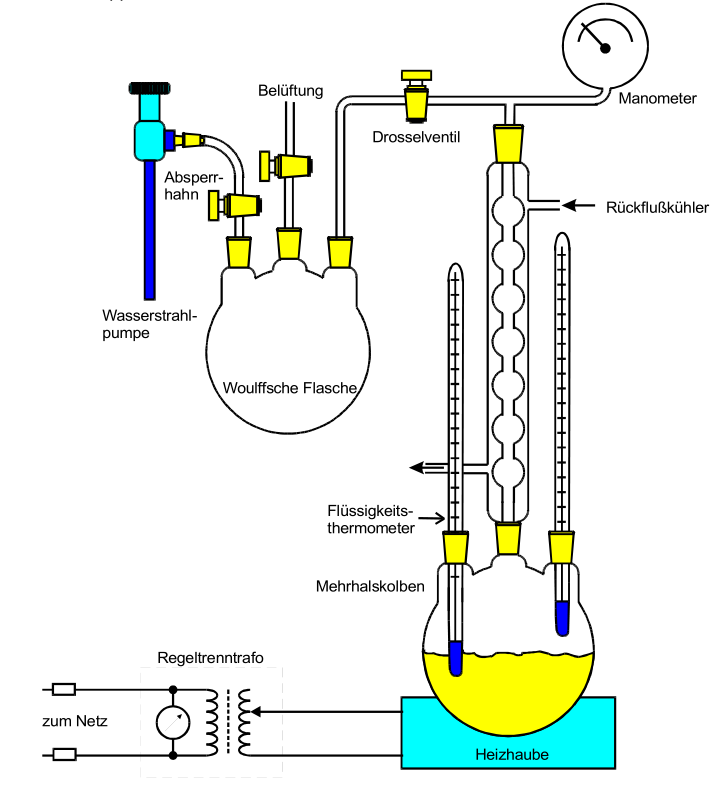
\includegraphics[width=\textwidth]{images/bild3.png}
    \caption{Versuchsaufbau zur Bestimmung einer Dampfdruck-Kurve für $30$ bis $\SI{70}{\milli\bar}$ \cite{V203}}
    \label{fig:skizze_3}
\end{figure}

Zunächst wird die ganze Apperatur evakuiert, dafür wird die Belüftung der Woulffschen Flasche geschlossen, um den Luftstrom zu unterbrechen.
Das Drosselventil, der Zugang zum Rest der Apperatur, wird geöffnet.
Der Absperrhahn, wird ebenfalls geöffnet, damit die Wasserstrahlpumpe das Gefäß evakuieren kann.
Ein angeschlossenes Manometer misst den Druck innerhalb der Apperatur, irgendwann wird dieser Druck nicht weiter fallen.
Dies sollte etwa im Bereich $30$ bis $\SI{70}{\milli\bar}$ geschehen, dann werden Absperrhahn und Drosselventil geschlossen und danach die Wasserstrahlpumpe abgeschaltet.
Das eigentliche Experiment beginnt mit dem Einschalten der Heizhaube, das Wasser in der Mehrhalshaube wird sich jetzt langsam erhitzen.
Gleichzeitig wird auch die Kühlwasserzufuhr eingeschaltet.
Das Wasser beginnt zu sieden, ein Teil des Wassers verdampft.
Das Thermometer, welches den Dampfbereich des Kolbens misst, wird als Temperaturmessung genutzt.
Immer wenn dort die Temperatur $T$ um $\SI{1}{\celsius}$ ansteigt, wird sie zusammen mit dem am Manometer abgelesenen Druck $p$ notiert.
Dabei wird die Kühlwasserzufuhr mit der Zeit immer weiter reduziert.
Dieser Prozess wird solange fortgeführt, bis der Druck auf $\SI{1000}{\milli\bar}$ angestiegen ist.

\subsection{Bestimmung einer Dampfdruck-Kurve im Hochdruckbereich}
\label{ssec:Db}

Damit der Druckbereich oberhalb von $\SI{1}{\bar}$ untersucht werden kann, wird eine andere Apperatur verwendet, da der Druck ansonsten zu hoch werden würde.
Eine mögliche Apperatur ist in \autoref{fig:skizze_4} dargestellt.

\begin{figure}
    \centering
    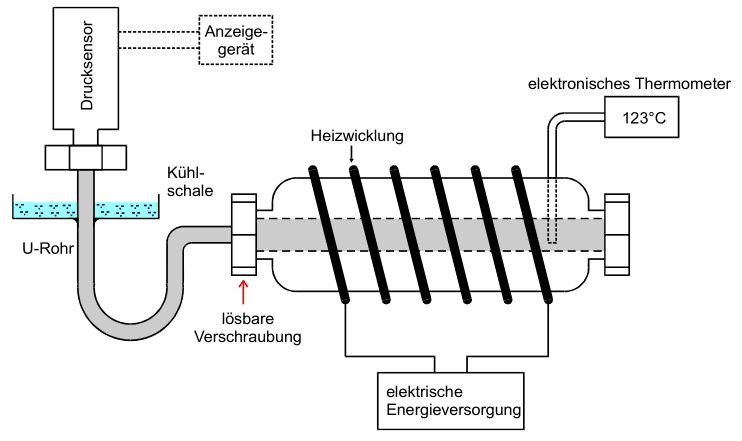
\includegraphics[width=\textwidth]{images/bild4.png}
    \caption{Versuchsaufbau zur Bestimmung einer Dampfdruck-Kurve für $p > \SI{1}{\bar}$ \cite{V203}}
    \label{fig:skizze_4}
\end{figure}

Bei dem durchgeführten Experiment, wurde keine Heizwicklung verwendet, sondern einige Heizstäbe unterhalb des Stahlzylinders, was aber zum gleichen Ergebnis führt.
Die Hitzezufuhr wird eingeschaltet, das Innere erhitzt sich also immer weiter.
An dem Thermometer kann die Innentemperatur abgelesen werden und an dem Manometer der entsprechende Druck.
Ab grob $\SI{100}{\celsius}$ beginnt der Druck zu steigen, wenn das passiert beginnt die eigentliche Messung.
Immer wenn der Druck um $\SI{0.5}{\bar}$ ansteigt, wird der Druck $p$ und die Temperatur $T$ notiert.
Wenn ein Druck von $\SI{15}{\bar}$ erreicht wurde, wird die Messung gestoppt und die Hitzequelle abgestellt.